In this section we conducted our experiments on public cloud using Amazon EC2 and private cloud using DAS-4 (the Distributed ASCI Supercomputer 4)~\cite{das4}. DAS-4 is the Dutch Computational Infrastructure, a six-cluster wide-area distributed system designed by the Advanced School for Computing and Imaging (ASCI) with research purposes.  We compare the degree of SLA fulfillement and resource consumption for each one of the resource provisioning mechanisms included in ConPaaS.

Note that, since DAS-4 is a homogeneous infrastructure, the profiling techniques were only evaluated on a heterogeneous platform like Amazon EC2. 

\fixme{Public cloud or Homogeneous infrastructure ??} 

\subsection{Testbed configuration}

As a realistic and representative scenario, we deployed Mediawiki application on both clouds using ConPaaS, and we ran the Wikibench tools utilizing Wikipedia workload traces.  To provide the Wikipedia services, an initial configuration was composed of 4 VMs, and 1 VM to host the Wikibench tools. The 4 VMs include a PhP service manager, a FPM-PhP agent, a Web server and a Http-proxy agent, and a MySQL service agent containing the English Wikipedia article data.

As we detailed, our system will scale out and back the number of VMs hosting FPM-PhP agents to guarantee the SLO (Service Level Objective). Initially, we fixed two SLOs one of 700ms (miliseconds) at platform's side and another of 1500ms at client's side. Our measurements shows the behavior of the Wikipedia services during 24h under a workload generated from real traces. Note that, our experiments only focus on the PhP response time and the resource consumption for our algorithms. The response time of static files were not taken into account due to its lightweight. 

\subsection{Public Cloud}

Our experiments on DAS4 relies on OpenNebula as IaaS, and used small instances for the PhP service (manager and agents) and a medium instance for the MySQL service (agent). OpenNebula's small instances provision VMs equipped with 1 CPU of 2Ghz, and 1GB of memory, while medium instances are equipped with 4 CPU's of 2Ghz, and 4GB of memory.

Figure~\ref{naiveDas4} and Figure~\ref{historyDas4} show the degree of SLA fulfillement for the naive and history algorithms on public clouds, indicating the average of response times obtained during the execution of one Wikipedia trace. The results show as the naive provisioning algorithm tend to generate more SLA violations due to its excesive reactive behavior. As we mentioned, this algorithm is an easy target to flash crowds effects, as a new VM can be added or removed  when having temporal and important variations of user requests. In contrast, Figure~\ref{historyDas4} shows a more stable behavior during the whole experiment, there is a 1% less of SLA violations (regarding the amount of PhP pages served).

\begin{figure}
\begin{center}
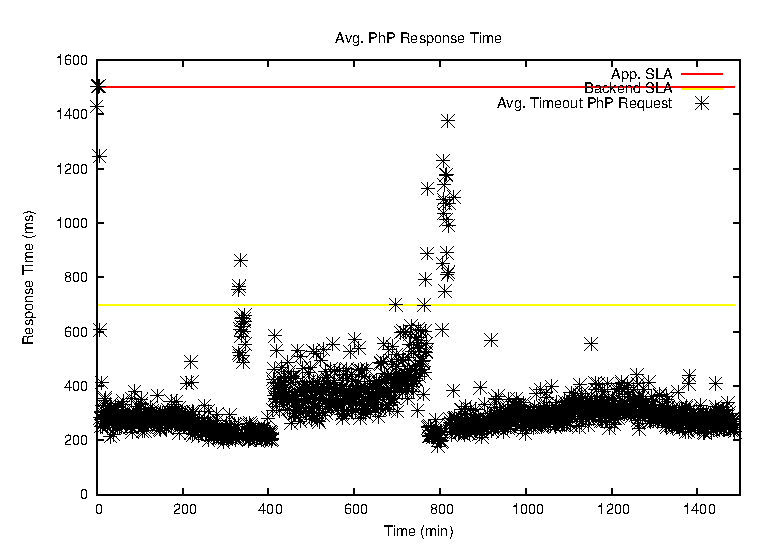
\includegraphics[width=0.49\textwidth, height=6cm]{./images/homogeneous/avgTimeout_PhP_naive}
\end{center}
\label{naiveDas4}
\caption{Avg. PhP resp. time on DAS4 -- Naive.}
\end{figure}

To better understand the behavior of both algorithms, we may focus on the resource consumption, as depicted on Figure~\ref{resComDas4}. The excesive reactive behavior of the naive alg. is illustrated in 350min and 800min, it  scaled back twice the system under-provisioning it during short periods of time. These actions increase the unstability of the application as well as the expenses. Our algorithm makes provisioning decision by analyzing workload's trend during the last few minutes, and thereby a more efficient resource usage has been done. VMs were added and removed during the period of time on which the Wikipedia workload presented important and constant variations of request rate, as depicted on Figure~\ref{workload}.

\begin{figure}
\begin{center}
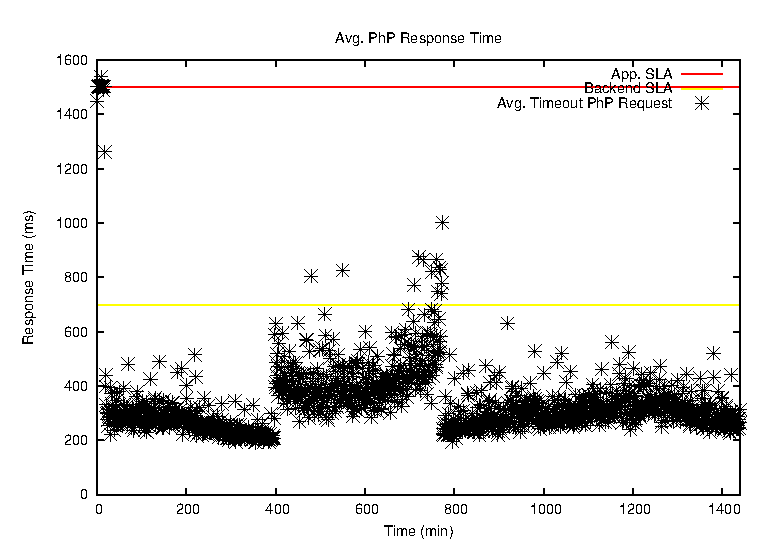
\includegraphics[width=0.49\textwidth, height=6cm]{./images/homogeneous/avgTimeout_PhP_history}
\end{center}
\label{historyDas4}
\caption{Avg. PhP resp. time on DAS4 -- History.}
\end{figure}

\begin{figure}
\begin{center}
\includegraphics[width=0.49\textwidth, height=5cm]{./images/homogeneous/numMachinesComp}
\end{center}
\label{resComDas4}
\caption{Resource consumption on DAS4.}
\end{figure}

\subsubsection{Discussion}

Using threshold-based algorithms, the performance follows an irregular pattern similar to the web traffic that produces an increment in the number of SLA violations. Its reactive behavior forces to the system to easily add and remove VMs affecting to the performance instead of improving it, and as a consequence these algorithms are wasteful regarding the resource usage. Unlike, the benefits behind of the history-aware are an efficient resource consumption and a regular performance pattern while meeting the application's SLA. 

Both algorithms are best-effort regarding the SLA fulfillement, and thereby short peaks in the workload (around of 5min.) are not covered. The heterogeneity of the PhP pages, containing images and requiring multiple Db queries, are in part responsible of isolated SLA violations during the execution..

It avoid to under-provisioning in two occasions  while decreases the number of SLA violation. However, tha naive alg. is vulnerable to temporal bursty workload variations (10 min), an increment of SLA violated is caused by under-provisioning operations in conjuction with workload variations. 



\subsection{Private Cloud}

Our experiments on EC2 used small instances for the PhP service (manager and agents) and  a medium instance for the MySQL service (agent). EC2 small instances provision VMs equipped with 1 EC2 CPU, and 1.7GiB of memory, while medium instances are equipped with 2 EC2 CPU's, and 3.75GiB of memory.

In the following, we analysis the behavior of our algorithms when taking provisiong decisions on a heterogeneous infrastructure. Figure~\ref{naiveEC2}, Figure~\ref{historyEC2} and Figure~\ref{historyWeightEC2} show the workload for the naive, history and history-weight algorithms respectively. As depicted on Figure~\ref{naiveEC2}, the naive algorithm presents an irregular performance pattern which is the result of a high frecuency of scaling operations. In particular, two peaks of workload caused in 300min and 820min are explained from the variations on the Wikipedia workload. However, there is a third peak of workload that corresponds to the period of time on which the workload significantly decreased. It explains the inherent degradation of the SLA fulfillement associated to frecuent scaling operations. 

On the other hand, Figure~\ref{} and Figure\ref{} show as the history and history-weight algorithm present a similar behavior. Even though both algorithms are best-effort, there is an important reduction in terms of SLA violation during the whole experiment.

\begin{figure}
\begin{center}
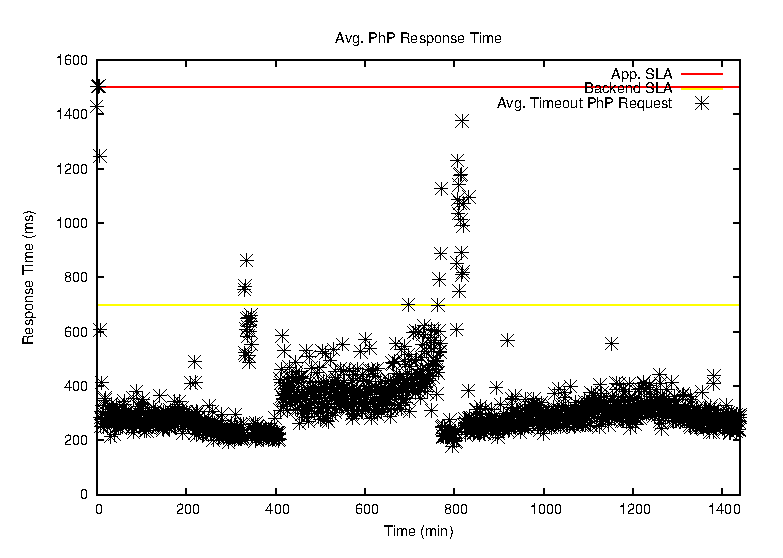
\includegraphics[width=0.49\textwidth, height=6cm]{./images/heterogeneous/avgTimeout_PhP_naive}
\end{center}
\label{naiveEC2}
\caption{Avg. of  response time on EC2 -- Naive.}
\end{figure}


\begin{figure}
\begin{center}
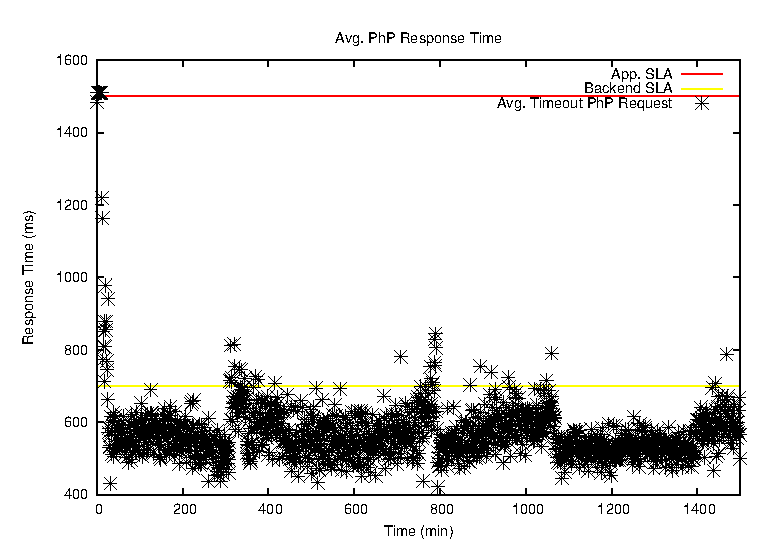
\includegraphics[width=0.49\textwidth, height=6cm]{./images/heterogeneous/avgTimeout_PhP_history}
\end{center}
\label{historyEC2}
\caption{Avg. PhP resp. time on EC2-- History.}
\end{figure}

\begin{figure}
\begin{center}
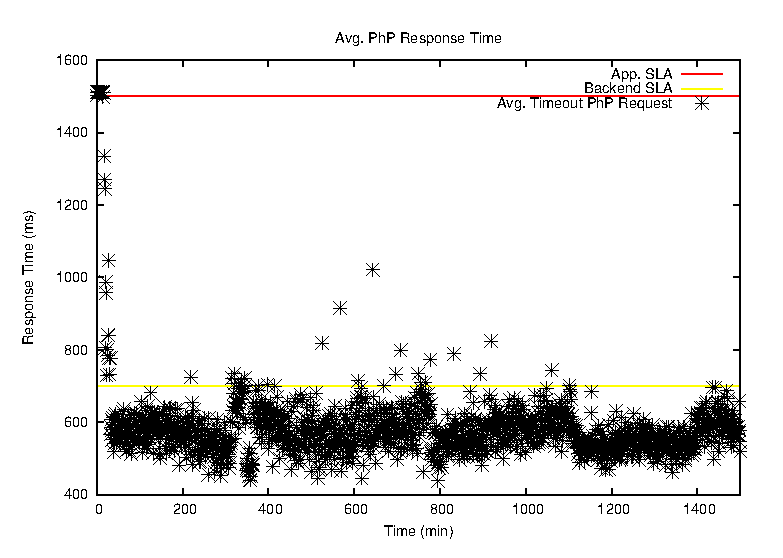
\includegraphics[width=0.49\textwidth, height=6cm]{./images/heterogeneous/avgTimeout_PhP_weightHistory}
\end{center}
\label{historyWeightEC2}
\caption{Avg. PhP resp. time on EC2-- Weight-History.}
\end{figure}

\begin{figure}
\begin{center}
\includegraphics[width=0.49\textwidth, height=5cm]{./images/heterogeneous/numMachinesCompEC2}
\end{center}
\caption{Resource consumption on EC2.}
\end{figure}


\subsubsection{Discussion}

\subsection{Discussion}

Consider the startup of VM to run an experiment.

The difference btw infrastructures as they present differnt performance and resource consumption.

 they are wasteful regarding the resource usage. providers use them to gain money.


